\documentclass{article}
\usepackage[T1]{fontenc}
\usepackage{lmodern}
\usepackage{graphicx}
\usepackage{amsmath,amssymb}
\usepackage[a4paper,margin=2cm]{geometry}
\usepackage[absolute,overlay]{textpos}
\setlength{\TPHorizModule}{1mm}
\setlength{\TPVertModule}{1mm}
\usepackage[indonesian]{babel}
\usepackage{hyperref}
\setlength{\emergencystretch}{2em}
% unit: Halaman 21

\begin{document}

% === Halaman 21 (python/native) ===

21

Cipherteks pada putaran terakhir 

disimpan di dalam A dan B. 

Gabungan keduanya adalah blok 

cipherteks yang berukuran 64 bit. 

Ai  - 1

Bi  - 1

S2i

S2i  + 1

Ai

Bi

for i  1 to r do

       A  ((A  B) <<< B) + S[2i]

       B  ((B  A) <<< A) + S[2i+1]

endfor

Proses enkripsi satu putaran:

% deskripsi: gambar native xref 112
\noindent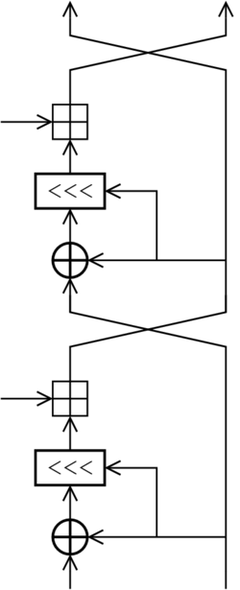
\includegraphics[width=0.85\textwidth]{../../images/python/page_021_img_01.png}

\end{document}
